\section{Versuchsdurchführung}
\label{sec:durchfuerung}

Die in Abb. \ref{fig:zirkulationsapparatur} dargestellte Zirkulationsapparatur wurde im ersten Teil des Versuches mit etwa \SI{65}{\milli\liter}reinem Ethanol befüllt. Es ist darauf zu achten dass alle Hähne verschlossen sind. Die Kühlwasserzufuhr für den Kondensator wurde freigegeben und die elektrische Heizung eingeschaltet. Die an der Heizung anliegende Spannung darf die \SI{180}{\volt } nicht übersteigen. Am elektrischen Thermometer wird die Temperatur der siedenden Flüssigphase abgelesen. Vor jeder Probennahme ist auf die Ausbildung des thermischen Gleichgewichtes zu warten und die Heizung abzustellen. Die Probennahme muss anschließend zügig durchgeführt werden. Dazu wird die für diesen Zweck vorgesehene und beschriftete Spritze in den jeweiligen Siphon herab gesenkt und etwa \SI{1}{\milli\liter} der Flüssigkeit angesaugt. Dabei wird die Probe für Flüssige Phase aus dem Siphon (3) und die Probe für die kondensierte Dampfphase aus dem Siphon (4) gezogen. Anschließend ist das entfernte Volumen an Flüssigkeit durch eine entsprechende Menge der jeweils weniger enthaltenen Komponente zu ersetzen. Zu Anfang liegt reiner Ethanol vor, weswegen nach jeder Probennahme Cyclohexan zugegeben wird. Um den azeotropen Punkt zu umgehen wird das Ethanol-Cyclohexan-Gemisch nach der 7. Messung abgelassen und durch reines Cyclohexan ersetzt. Die Zirkulationsapparatur muss gründlich mit Druckluft ausgeblasen werden um Rückstände herauszuspülen, bevor das Cyclohexan eingefüllt werden kann. Das Vorgehen ist analog zu dem beim Ethanol. Die gezogenen Proben werden mit Hilfe eines Abbe-Refraktometers auf ihren Brechungsindex untersucht. Dazu wird die Lampe des Refraktometers eingeschaltet und die Probe in das dafür vorgesehene Loch am Probenträger eingespritzt. Mit Hilfe des rechten Stellrades und dem Blick durch das Reckte Okular wird ein klarer und möglichst scharfer Horizont eingestellt. Durch das linke Okular kann dann der Brechungsindex an der entsprechenden Skala abgelesen werden. Die Werte für den Brechungsindex von Flüssig- und Dampfphase werden zusammen mit der abgelesenen Temperatur in Tabellenform notiert. Die Rohdaten dieses Versuches sind zusammen mit den Berechnungsergebnissen auf dem Vordruck im Anhang einzusehen.
Die Abfälle sind in einen Sammelbehälter zu entsorgen. Nach Beendigung aller Messungen wird die Anlage heruntergefahren. Außerdem muss die Zirkulationsapparatur wieder entleert und ausgeblasen werden.
\begin{figure}[h!]
	\centering
	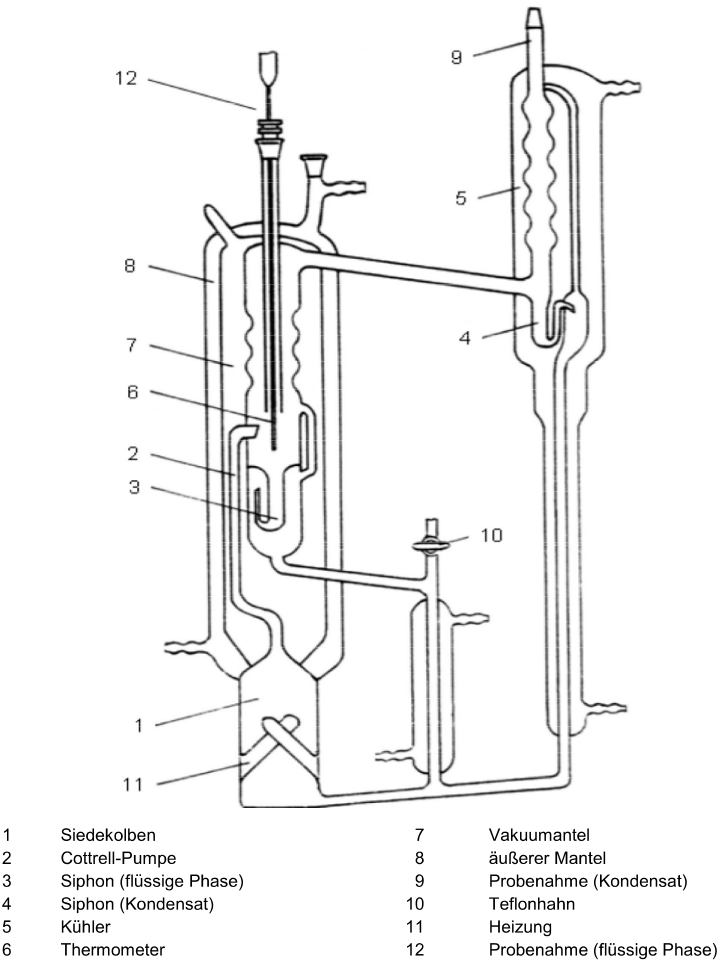
\includegraphics[width=0.7\linewidth]{img/zirkulationsapparatur}
	\caption{Beschrifteter Aufbau der Zirkulationsapparatur mit Legende}
	\label{fig:zirkulationsapparatur}
\end{figure}